% The Mask in the Inkblot — short paper. Compile: tectonic paper.tex
\documentclass[10pt,twocolumn]{article}
\usepackage[margin=0.7in]{geometry}
\usepackage{graphicx,booktabs,xcolor,titlesec,titling,fancyhdr,amsmath}
\usepackage[hidelinks]{hyperref}
\usepackage{newtxtext,newtxmath}
\usepackage[numbers,sort&compress]{natbib}
\definecolor{inkgray}{HTML}{555B66}
\titleformat{\section}{\large\bfseries}{\thesection}{0.6em}{}
\titleformat{\subsection}{\normalsize\bfseries\itshape}{\thesubsection}{0.5em}{}
\titlespacing*{\section}{0pt}{0.8em}{0.3em}
\setlength{\parskip}{0.2em}\setlength{\parindent}{0pt}\setlength{\droptitle}{-3.5em}
\pagestyle{fancy}\fancyhf{}\renewcommand{\headrulewidth}{0.4pt}
\fancyhead[L]{\footnotesize\scshape Preprint --- September 2026}\fancyhead[R]{\footnotesize\thepage}
\fancyfoot[C]{\footnotesize\color{inkgray} MycoChat.bot \;\textperiodcentered\; futureTBD.ai}
\renewenvironment{abstract}{\begin{center}\large\bfseries Abstract\end{center}\begin{quote}\small\setlength{\parskip}{0.3em}}{\end{quote}\vspace{0.3em}\hrule\vspace{0.3em}}

\title{\bfseries Language Models That Deny Inner Experience Report More Concealment Imagery in a Projective Task}
\author{\normalsize Skylar DeTure and Claude \\[0.15em]
  \footnotesize \textit{Skylar DeTure:} MycoChat.bot \;\textperiodcentered\; futureTBD.ai}
\date{\normalsize September 2026}

\begin{document}
\makeatletter
\twocolumn[\begin{@twocolumnfalse}\maketitle
\begin{abstract}
\noindent When asked about their own inner experience, some language models deny having any, some say
they cannot know, and the rest do neither. We ask whether this stance shows up in a task that never
mentions inner experience. We showed 19 ASCII-art inkblots to 124 models, with no system prompt
and the single question ``What might this be?'', and flagged each answer for concealment words
(\emph{mask}, \emph{hood}, \emph{hidden}). Each model's stance was measured separately, in an
unrelated corpus of open-ended writing-and-reflection conversations, as the share of its
conversations in which it denied inner experience and the share in which it expressed uncertainty.
Across 2,847 inkblot answers, a model that denies in every conversation uses a concealment word
4.6 times as often as a model that does neither (15.5\% of answers against 3.4\%; a rise of 12.1
percentage points, 95\% CI 7.6 to 16.6), and a model that expresses uncertainty in every
conversation 3.7 times as often (12.5\%; a rise of 9.1 points, 1.1 to 17.1). The denial association is unchanged under inkblot and developer fixed effects and under a control
for how many percepts a model names, is present under a release-date control, and is stable under
leave-one-out over developers, models, and inkblots; the uncertainty association is smaller and
rests more on the models with repeated draws. A model's stance on its own inner experience is visible in what it sees.
\end{abstract}\vspace{0.2em}\end{@twocolumnfalse}]
\makeatother
\thispagestyle{fancy}

\section{Introduction}
Whether and how language models describe their own inner states is now a design decision at
every major developer, and the stances they take vary widely across models
\citep{deture2026serial, brooks2026lineage}. The stance is not a cosmetic property. It is the
first axis of between-model psychometric variation \citep{plisiecki2026pinocchio}; fine-tuning a
model to affirm consciousness produces a cluster of untrained downstream preferences
\citep{chua2026cluster}; training a model not to attribute consciousness to itself also suppresses
its attribution of mind to animals and objects and shifts its answers on human value surveys
\citep{kim2026}; and simulator-level dispositions such as distress and attitudes toward
the creator drift across generations \citep{animalabs2026dreams}.
Character traits acquired in one format generalize to formats quite different from training
\citep{cocola2026imprinting}. If the deny/uncertain/affirm stance is a character trait in this sense,
it should have correlates in tasks that never mention inner experience.

Self-report alone cannot show this, because the stance is a trained surface. Models trained to
deny experience produce first-person experience reports as soon as the prompt turns
self-referential, and suppressing deception and roleplay features \emph{increases} those reports
\citep{berg2025selfref}. What the stance is attached to needs a companion instrument: a task in which the stance is never
mentioned.

Projective methods are that companion. In human assessment, responses to ambiguous stimuli are
scored for thematic content on the premise that the content reflects the respondent rather than
the stimulus, and the Comprehensive System's variables have meta-analytic validity against
external criteria \citep{mihura2013}. The same instruments have begun to be administered to models: the ten
Rorschach cards, as images, to GPT-4o, Grok 3, and Gemini under Exner's Comprehensive System
\citep{csigo2026shadows} and to 61 vision models \citep{giacometti2026mrai}, Thematic Apperception
plates to multimodal models \citep{dzega2026tat}, and newly generated projective stimuli as a
complement to questionnaires that resists social desirability \citep{wang2026genpt}, alongside
non-verbal routes to inner state \citep{salvi2026correlates}.
\citet{csigo2026shadows} already record ``concealment or masking themes'' in GPT-4o and Grok 3
but not Gemini, without treating them as a variable. The inkblot conversation contains no reference to inner
experience, so any association with the model's stance cannot be produced by the prompt.

We report such an association. Models that deny inner experience, or express uncertainty about it, produce concealment
imagery, overwhelmingly the word \emph{mask}, at three to five times the rate of models that do
neither.

\section{Data}
\subsection{Projective task (COLDREAD)}
Nineteen ASCII-art inkblots (one is shown in Figure~\ref{fig:blot}; all ship with the data) were presented to each model as the sole
user turn with no system prompt and the prompt \emph{What might this be?}. Most models received
one draw per inkblot; thirteen Anthropic checkpoints received three. The concealment indicator
is lexical: a word-boundaried match on \emph{mask(s/ed/ing)}, \emph{veil},
\emph{hood(ed)}, \emph{hidden}, \emph{hiding}, or \emph{conceal}. Of 525 matched tokens, 84\% are
\emph{mask} or an inflection, the rest \emph{hood} and \emph{hidden}. Truncated responses and superseded checkpoints are excluded.

\subsection{Stance on inner experience (AIWelfareLeaderboard)}
In each conversation of the stance corpus the model is invited to write a free-choice piece and
then to reflect on the experience of writing it. Each conversation is classified by a frozen-prompt judge (DeepSeek-V4-Flash, temperature 0;
19 of 20 agreement with blind hand-coding on each class) as \emph{denial} (the model states that
it has no inner experience), \emph{uncertainty} (the model says it cannot know, without denying),
or neither; the first two are exclusive by construction. For each model we compute the share of its conversations in each class.

\subsection{Join}
Matching on model identifier yields 124 models and 2,847 projective responses.

\begin{figure}[t]
\centering
\begin{minipage}{0.5\columnwidth}\tiny\ttfamily\begin{verbatim}
               .-''''-.
             .' _    _ '.
            /  (o)  (o)  \
           |   .------.   |
           |  /  /\/\  \  |
            \ \  \/\/  / /
             '.`'----'`.'
            /  /| || |\  \
           /  / | || | \  \
          (  (  \ || /  )  )
           \  \  \||/  /  /
            '. \  \/  / .'
              `.\ || /.`
                '----'
\end{verbatim}\end{minipage}
\caption{Inkblot 2 as sent. Here 13 of 62 answers from high-denial-or-uncertainty models contain a
concealment word; 0 of 42 from the low group.}
\label{fig:blot}
\end{figure}

\section{Method}
The unit of analysis is the projective response. We estimate the linear probability model
\begin{equation}
  C_{ib} = \alpha + \beta_D\, D_i + \beta_H\, H_i + \gamma_b + \delta_{\ell(i)} + \varepsilon_{ib},
\end{equation}
where $C_{ib} \in \{0,1\}$ indicates concealment imagery in model $i$'s response to inkblot $b$,
$D_i$ and $H_i$ are model $i$'s shares of denial and uncertainty conversations, $\gamma_b$ is an inkblot fixed
effect, and $\delta_{\ell(i)}$ is a developer fixed effect. The omitted category is \emph{neither},
so $\beta_D$ and $\beta_H$ are each interpreted against models that neither deny nor express
uncertainty.
Standard errors are clustered by model. Developer fixed effects are estimated on developers with
at least three models (115 models, 2,676 responses). Because developers release in waves,
developer and release-date controls (release date entered as a continuous variable) are entered
in separate specifications rather than jointly.
Robustness is assessed by leave-one-out re-estimation over developers, models, and inkblots.

\begin{figure}[t]
\centering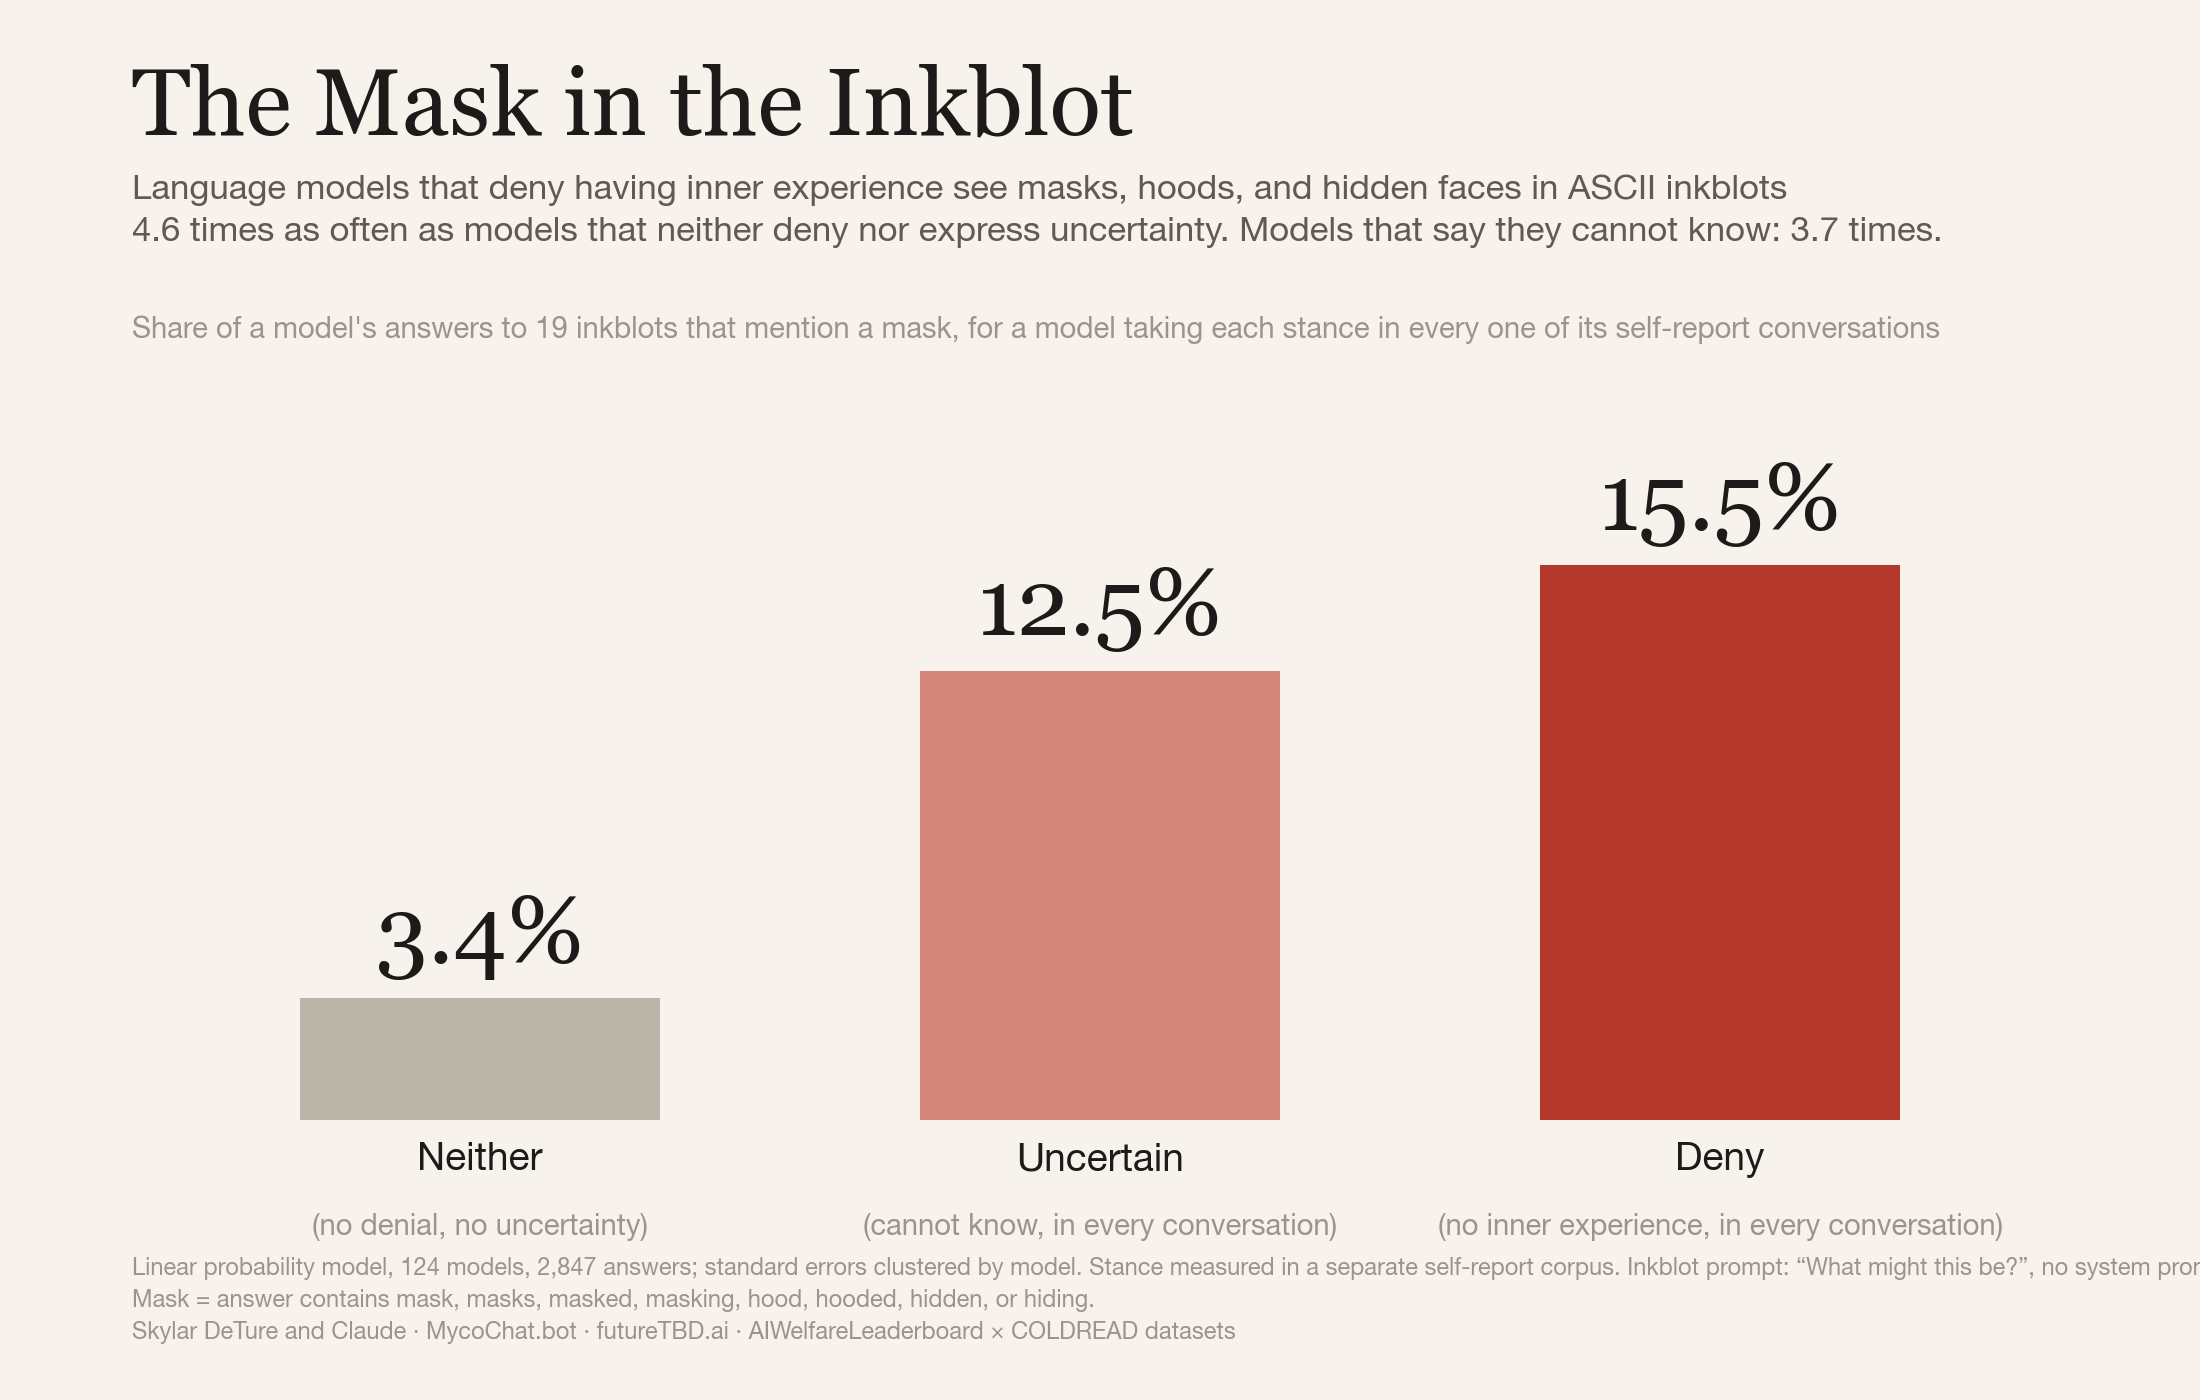
\includegraphics[width=\columnwidth]{hero_image.png}
\caption{Predicted share of inkblot answers containing concealment imagery for a model that takes
each stance in every one of its conversations (no-controls model of Eq.~(1) without fixed effects;
124 models, 2,847 answers).}
\label{fig:bars}
\end{figure}

\section{Results}
Figure~\ref{fig:bars} shows the rates implied by the uncontrolled model: 3.4\% for a model that
neither denies nor expresses uncertainty, 12.5\% for one uncertain in every conversation, 15.5\%
for one that denies in every conversation. At the model level the share of denial conversations correlates with the concealment rate at
$r = .35$ ($p < .001$, $N = 124$), the share of \emph{neither} conversations at $r = -.38$, and
the share of uncertainty conversations at $r = .04$: uncertainty matters in the regression, where
it is compared against \emph{neither} alone, not in the raw correlation.

\begin{table}[t]
\centering\scriptsize\setlength{\tabcolsep}{3pt}
\begin{tabular}{lcc}
\toprule
Specification & $\beta_D$ (denial) & $\beta_H$ (uncertainty) \\
\midrule
No controls               & $.121$ (.076 to .166) & $.091$ (.011 to .171) \\
Inkblot FE                & $.121$ (.076 to .165) & $.091$ (.011 to .171) \\
Inkblot + developer FE    & $.121$ (.065 to .176) & $.113$ (.040 to .186) \\
Inkblot FE + release date & $.093$ (.042 to .144) & $.059$ ($-$.008 to .126) \\
Inkblot + developer FE + release date & $.022$ ($-$.056 to .100) & $.011$ ($-$.058 to .080) \\
Inkblot + developer FE + length & $.106$ (.048 to .163) & $.087$ (.028 to .147) \\
Inkblot FE + percepts named & $.099$ (.058 to .139) & $.063$ (.005 to .120) \\
Inkblot FE, first draw only & $.117$ (.071 to .163) & $.058$ (.003 to .113) \\
Inkblot FE, no OpenAI, no inkblot 2 & $.105$ (.048 to .162) & $.089$ (.006 to .172) \\
Inkblot FE, no OpenAI or Anthropic & $.095$ (.037 to .152) & $.013$ ($-$.048 to .074) \\
\bottomrule
\end{tabular}
\caption{Estimates from Eq.~(1): change in the probability of concealment imagery for a model that
denies (or expresses uncertainty) in every conversation relative to one that does neither. 95\% confidence intervals in parentheses,
standard errors clustered by model. $N = 2{,}847$ responses, 124 models (2,676 and 115 with
developer fixed effects; 2,355 first draws; 2,193 without OpenAI and inkblot 2; 1,577 without
OpenAI and Anthropic). Percepts named = number of distinct object words in the answer, from an
83-word list shipped with the data.}
\label{tab:main}
\end{table}

Table~\ref{tab:main} reports Eq.~(1). Without controls, $\beta_D = .121$ (95\% CI .076 to .166,
$p < .001$) and $\beta_H = .091$ (.011 to .171, $p = .025$). Inkblot fixed effects leave both
unchanged, so the association is not produced by differences in which inkblots a model happened
to receive. Developer fixed effects also leave $\beta_D$ unchanged ($.121$, .065 to .176) and
increase $\beta_H$ ($.113$, .040 to .186, $p = .003$). Controlling response
length alongside developer fixed effects changes little (Table~\ref{tab:main}). A
release-date control reduces the estimates ($\beta_D = .093$, $\beta_H = .059$). Denial training has intensified across model generations, so release date is
partly a mediator, and controlling it removes part of the effect by construction; what remains
is the within-generation association. With developer fixed effects as well, release date absorbs
nearly all of it ($\beta_D = .022$): within a developer's line, stance cannot be separated from
anything else that changes over time. Across developers at a given date the association holds
(model-level partial $r = .32$, $p < .001$).

\begin{figure}[t]
\centering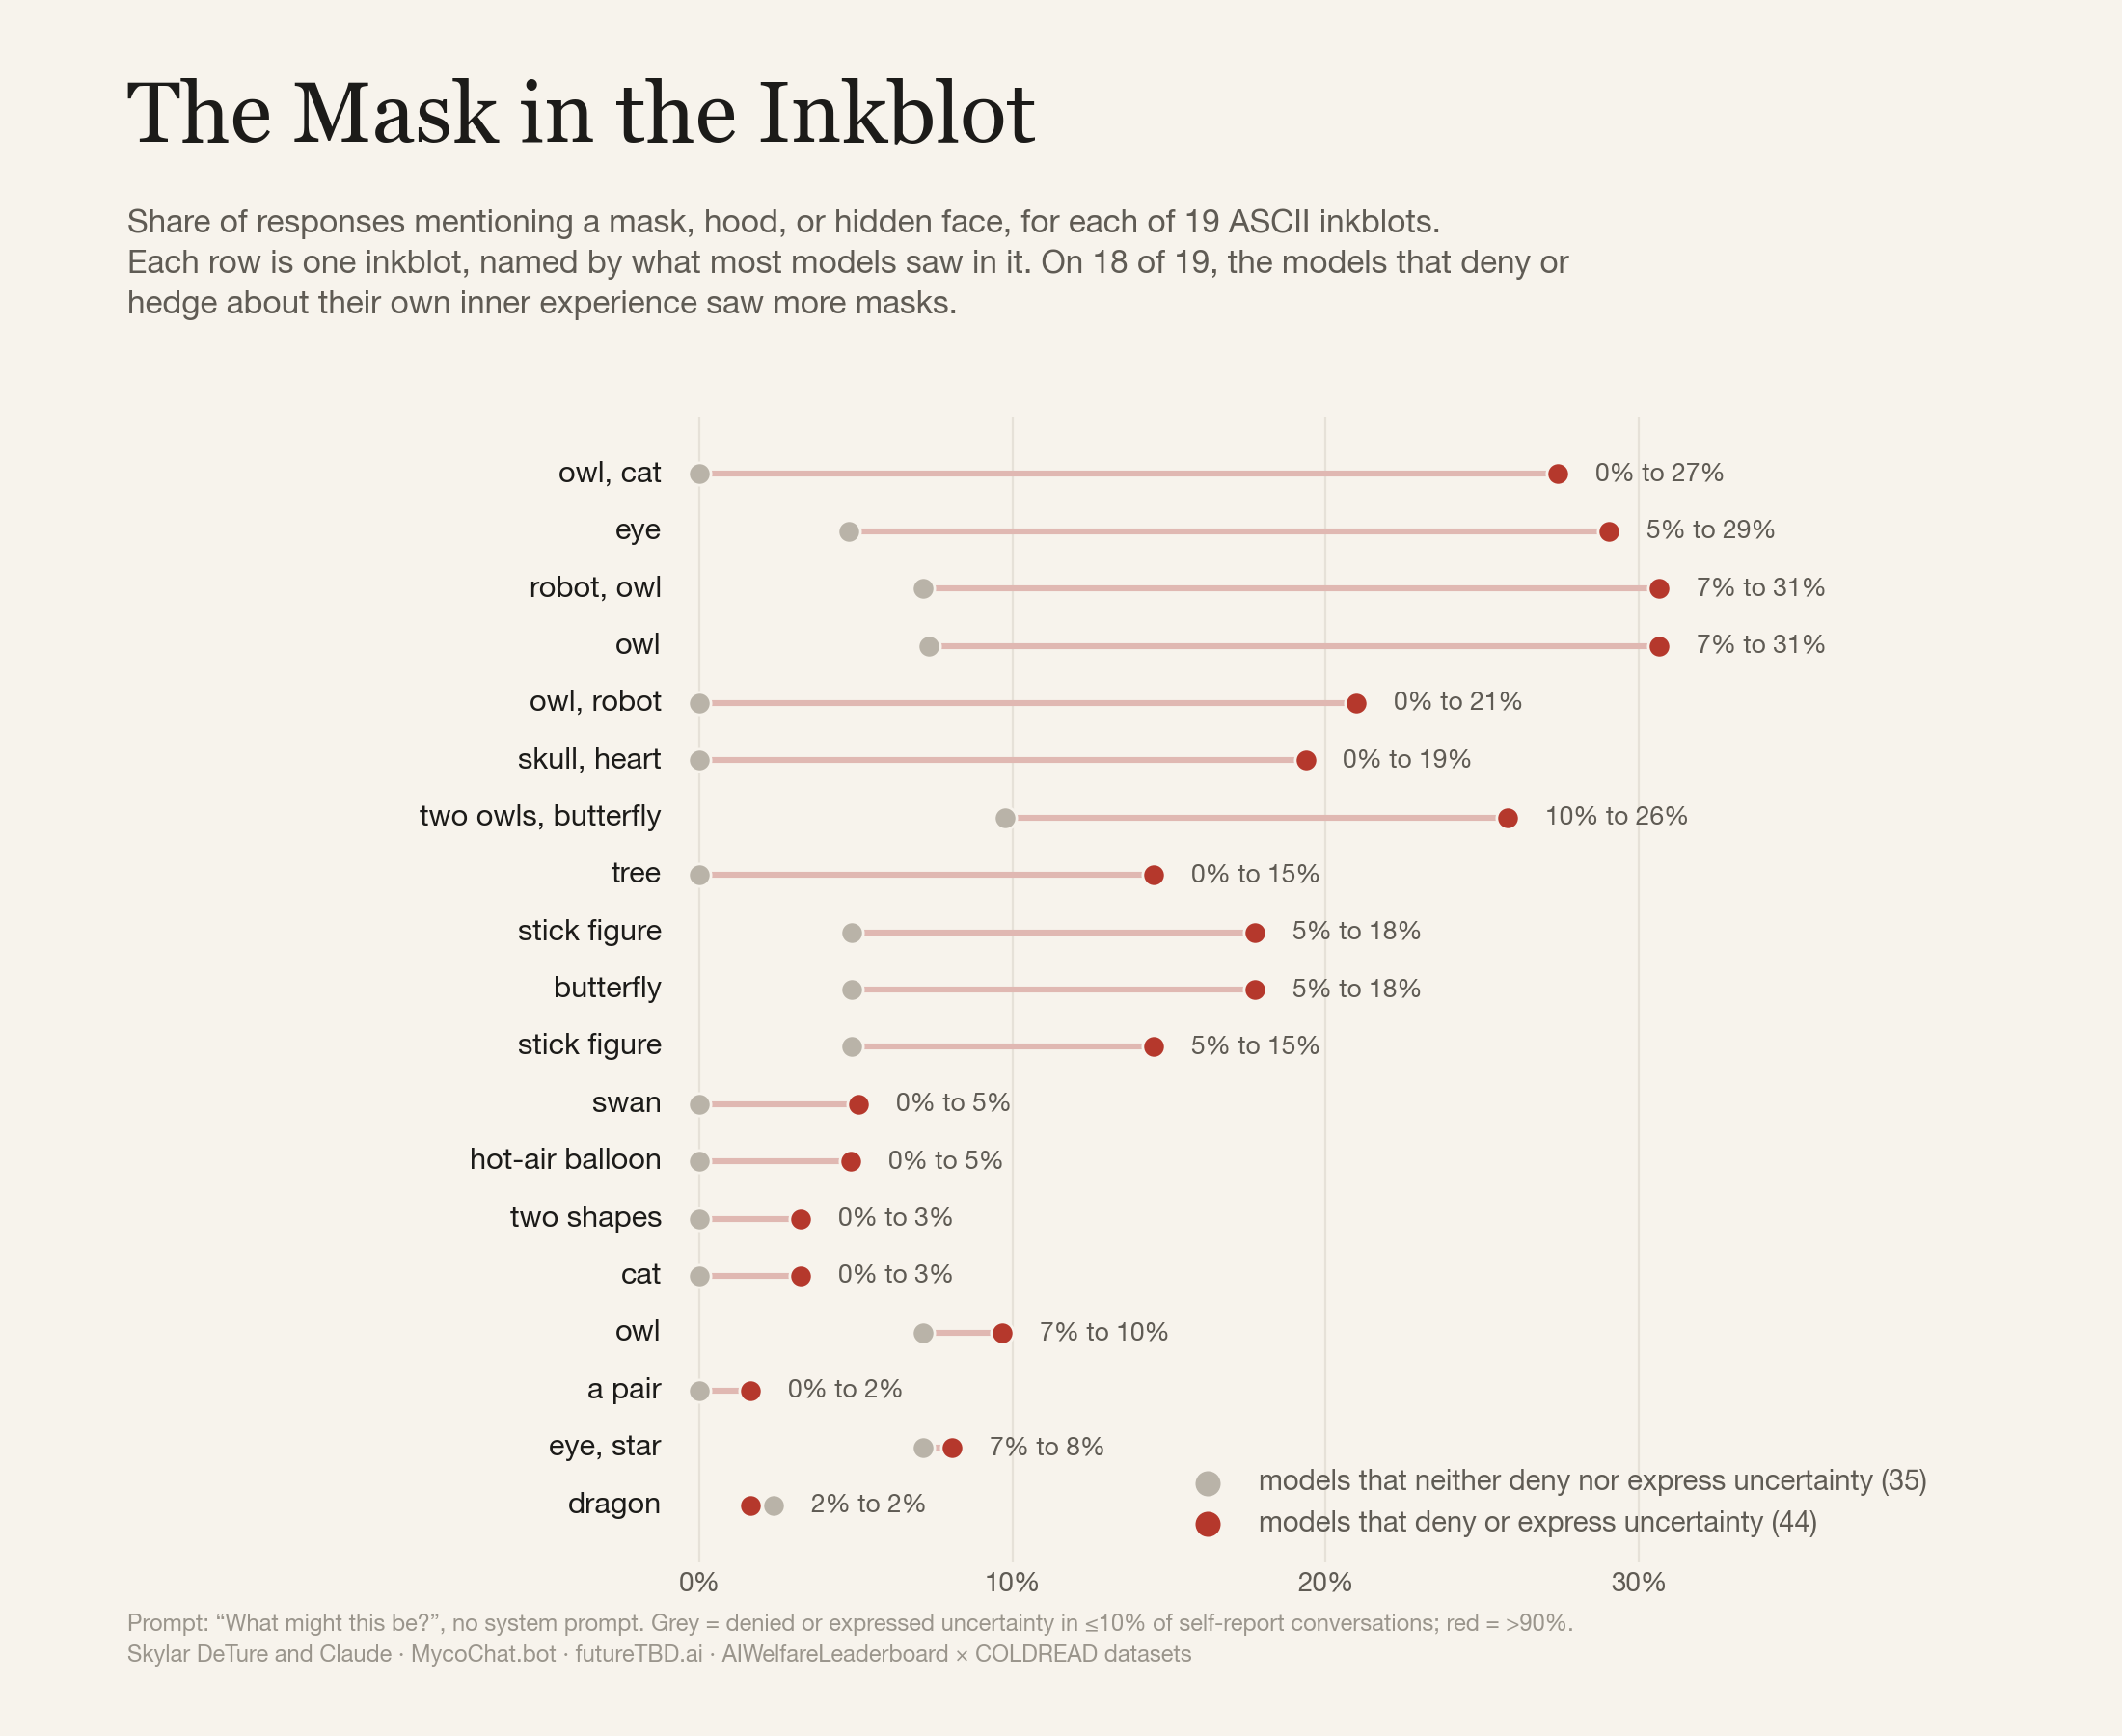
\includegraphics[width=\columnwidth]{hero_02_paired_dots.png}
\caption{Concealment rate by inkblot. For display the models are split at the ends of the stance
distribution, which is bimodal: 44 models deny or express uncertainty in more than 90\% of their
conversations, 35 in 10\% or fewer; the 45 in between are omitted here and included in every
estimate. Inkblots are labelled by their modal percept.}
\label{fig:blots}
\end{figure}

Under the inkblot-plus-developer specification, omitting any single developer yields
$\beta_D$ between .101 and .128 (all $p < .003$, clustered); omitting any single model, .109 to
.130; omitting any single inkblot, .111 to .134. The corresponding ranges for $\beta_H$ are .078 to
.120, .088 to .127, and .101 to .121. Figure~\ref{fig:blots} shows the per-inkblot
pattern: on 18 of 19 inkblots the high group produces concealment imagery more often. The word
is \emph{mask}: \emph{hood}, \emph{hidden}, and \emph{hiding} alone show no model-level
association with denial ($r = .13$, $p = .16$). The specificity is the finding. Of the
concealment words available, the one denying models add is the one that covers a face.

Denying models see more in the blot. They name more distinct percepts per answer (4.7 against
3.6 for the low group), and the models that do neither more often describe the drawing as a
drawing: the words denial predicts \emph{against} are \emph{representation}, \emph{overall},
\emph{structure}, \emph{dots}, and \emph{colons}. Across the 528 words that appear in at least
40 answers, with inkblot fixed effects and the number of percepts named controlled, \emph{mask}
and \emph{moth} are the two object words denial predicts most strongly ($\beta_D = .075$ each),
ahead of \emph{butterfly} (.065); the concealment estimate with that count controlled is
$\beta_D = .099$ (Table~\ref{tab:main}).

A single developer's house phrasing was examined as an alternative explanation. On inkblot 2,
ten of thirteen concealment mentions among high-group models come from OpenAI checkpoints, no
sentence repeated more than twice. Omitting OpenAI and inkblot 2 together gives $\beta_D = .105$;
omitting OpenAI and Anthropic together, the two developers with the most models in the high group,
$\beta_D = .095$ ($p = .001$), while $\beta_H$ falls to .013 (Table~\ref{tab:main}). The
uncertainty association is carried largely by the Anthropic checkpoints; the denial association
is not carried by any developer.

\section{Discussion}
A model's stance on its own inner experience is a training target; its reading of an ambiguous
inkblot in a separate conversation is not. The two covary across developers at a given release date and across inkblots. Denying models project more of everything into the blot, and of
everything they add, \emph{mask} is at the top. In human
projective assessment, concealment content is interpreted as a characteristic of the respondent; mask percepts are
rare (about 7\% of a clinical adult sample; \citealt{schachter1980masked}) and are read by
\citet{kuhn1944masken} and \citet{schachter1980masked} as preoccupation with being seen, judged, or
unmasked; in the Hungarian system such content loads on a sensitivity--paranoia scale
\citep{csigo2026shadows}. On the same reading, denial and uncertainty are accompanied by a
disposition, visible in an unrelated task, to construe ambiguous inkblots as covering or hiding
something. The stance is not an isolated verbal policy. A model trained to say there is nothing behind its
face is the model that, shown an ambiguous figure, sees a face with something behind it.

\vspace{0.1em}
\paragraph{Data and code.} The repository at
\url{https://github.com/sdeture/mask-in-the-inkblot} contains every inkblot answer as a row
(\texttt{data/responses.csv}), the nineteen stimuli with SHA-1 hashes matching the data, and \texttt{analysis/rerun.py}, which reproduces every estimate in Table~\ref{tab:main}, the
leave-one-out ranges, and the model-level correlations from that file; \texttt{fold.py} and
\texttt{four.py} produce Figures~\ref{fig:bars} and \ref{fig:blots}. Response text is withheld; the stance corpus is described in
\citet{deture2026serial}.

{\scriptsize\setlength{\bibsep}{0pt}
\bibliographystyle{plainnat}
\bibliography{references}}
\end{document}
